\documentclass[a4paper,11pt,twocolumn]{article}
\usepackage[utf8]{inputenc}
\usepackage[top=1.8cm,bottom=2.0cm,right=1.35cm,left=1.35cm,columnsep=0.5cm]{geometry}
\usepackage{setspace, url}
\usepackage[natbibapa]{apacite}
\bibliographystyle{apacite}
\usepackage{graphicx}
\usepackage{amsmath}
\usepackage{amsfonts}
\usepackage{amssymb}

\usepackage{lipsum}% this geenerates fictitious text for sample
%opening
\title{A study of non-linear dimensioanlity reduction methods}
\author{A. Good Student \\
        School of Computing and Information Technology\\
        University of Wollongong\\
        CSCI933, SN:1234567, \url{ags123@uowmail.edu.au}}
\date{May 2, 2020}

\begin{document}
\onehalfspacing
\twocolumn[
  \begin{@twocolumnfalse}
    \maketitle
    \begin{abstract}
   In this report we study four dimensionality methods and compare  their performances under a  classification task. Specifically, we explored the performances for both artifically generated and naturral datasets. Under a 1-NN classification task it was found that linear methods perform better than their non-linear counterpart. 
    \end{abstract}
  \end{@twocolumnfalse}
]


\section{Introduction}
\label{sec:introduction}
Dimensinality reduction plays an important role in the analysis of data with high dimension. \cite{maaten2008} conducted a series of experiments to determine the extent to which the performances of the various dimensionality reduction techniques differ on artificial and natural datasets. An extended versio of the paper provides more details~\citep{maaten2009}.
\lipsum[2]
\section{Theory and properties of techniques}
\lipsum[3]
\subsection{Principal Component Analysis (PCA)}

\lipsum[4]
\subsection{Kernel PCA}
We read about kernel methods in the book by \cite{taylor2004}.
\lipsum[1]
\subsection{Autoencoders}
\lipsum[2]
\subsection{Local linear embedding}
\lipsum[1]
\section{Experiments}
\lipsum[3]
\subsection{Experimental setup}
\lipsum[1]
\subsection{Artificial datasets}
\lipsum[2]
\subsection{Natural datasets}
\lipsum[3]
\subsection{Results - Artificial datasets}
\lipsum[1]
\begin{figure}[h!t]
    \centering
    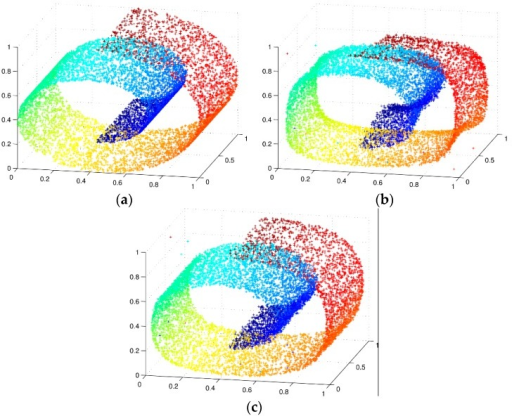
\includegraphics[scale=0.3]{swiss_roll.png}
    % swiss_roll.png: 512x416 px, 72dpi, 18.06x14.68 cm, bb=0 0 512 416
    \caption{An example of image inserted in report}
    \label{fig:swiss_roll}
\end{figure}
We have provided an image of the artifical data, \texttt{swiss roll} generated by our code in Figure~\ref{fig:swiss_roll}.

\subsection{Results - Natural datasets}
\lipsum[3]

\begin{table}[h!t]
\caption{Table showing results}
{%
\newcommand{\mc}[3]{\multicolumn{#1}{#2}{#3}}
\begin{center}
\begin{tabular}{lccccc}
× & \mc{5}{c}{Methods}\\\cline{2-6}
\mc{1}{l}{Dataset} & \mc{1}{c}{None} & \mc{1}{c}{PCA} & \mc{1}{c}{KPCA} & \mc{1}{c}{Autoenc} & \mc{1}{c}{LLE}\\\hline
Swiss roll & 1 & 2 & 3 & 4 & 5\\
Broken Swiss & 6 & 7 & 8 & 9 & 10\\
Helix & 3 & 9 & 10 & 7 & 6\\
MNIST & 4 & 8 & 5 & 8 & 5\\
Olivetti face & 6 & 7 & 7 & 8 & 9
\end{tabular}
\end{center}
}%
\label{tab:results1}
\end{table} 
Table~\ref{tab:results1} summarises our results and will be discussed in Section~\ref{sec:discussion}


\section{Discussion}
\label{sec:discussion}
\lipsum[2]
\section{Conclusion}
\label{sec:conclusion}
\lipsum[9]
\bibliography{report_template}

\end{document}
